\documentclass[12pt, a4paper]{article}

\usepackage[utf8]{inputenc}
\usepackage{geometry}
\usepackage{hyperref}
\usepackage{graphicx}
\usepackage{xcolor}
\usepackage{titlesec}
\usepackage{parskip}

\geometry{margin=1in}

\begin{document}

\begin{titlepage}
    \centering
    \vspace*{2cm}
    
    \Huge
    \textbf{NexChat}
    
    \vspace{0.5cm}
    \LARGE
    Product Development Report
    
    \vspace{1.5cm}
    
    \textbf{Course:} \\
    Computer Systems and Design
    
    \vspace{2cm}
    
    \textbf{Group Members:} \\
    \Large
    Amathul Azeez Sarah \\
    Hirannya Mhaisbadwe \\
    Sanjani Kumari \\
    Aditya Jha
    
    \vfill
    
    \large
    \today
    
\end{titlepage}

\begin{abstract}
This report details the end-to-end development, architecture, and design of \textbf{NexChat}, a modern, real-time group messaging application. Built using a React frontend, a FastAPI Python backend, and native WebSockets, the application provides a seamless, low-latency chatting experience. This report discusses the product overview, UI/UX design, technology stack, and the decoupled client-server architecture developed for the Computer Systems and Design course.
\end{abstract}

\tableofcontents
\newpage

\section{Introduction}
NexChat was conceptualized as a lightweight, highly responsive chat application allowing multiple users to connect and interact in a shared room without page reloads. The primary goal of this project was to apply core principles of computer systems engineering to create a robust, full-stack application that leverages modern web technologies—specifically native WebSockets for bidirectional communication, bypassing the limitations of traditional HTTP polling.

\section{Overview}
NexChat serves as a centralized group communication platform. It is designed to be highly reliable, ensuring that users do not lose their connections or chat history unintentionally.

\subsection{Key Product Features}
\begin{itemize}
    \item \textbf{Real-Time Messaging:} Lightning-fast communication powered by native WebSockets ensuring zero-latency message delivery.
    \item \textbf{Smart Session Management:} A custom heartbeat mechanism allows users to briefly close their browser or switch tabs (within a 5-minute window) without losing their session or chat history.
    \item \textbf{Tab Deduplication:} Prevents ghost connections. If a user opens a new tab, the backend detects the active session token and safely disconnects the old tab, maintaining only one active connection per user.
    \item \textbf{Live Roster:} A real-time updating list of online users with connection status indicators.
    \item \textbf{Inline Replies:} Users can reply to specific messages, creating a clear conversational thread.
\end{itemize}

\section{Design}
The user interface was built completely from scratch, without reliance on heavy third-party CSS frameworks, to ensure maximum performance and complete design control.

\subsection{UI/UX Principles}
\begin{itemize}
    \item \textbf{Design System:} We established a rigid set of CSS variables (\texttt{--clr-bg}, \texttt{--clr-accent}, etc.) to ensure visual consistency across all components.
    \item \textbf{Theming:} A dynamic hook intercepts theme toggles and maps a \texttt{data-theme="light"} attribute to the root HTML element, instantly flipping the application between Dark and Light modes.
    \item \textbf{Visual Aesthetics:} Glassmorphism was utilized in the login card via strict box-shadows, combined with CSS \texttt{mix-blend-mode} and custom keyframe animations (\texttt{@keyframes msgIn}) for smooth message appearance.
\end{itemize}

\subsection{Design Scenario Walkthrough}
To demonstrate the application design and user flow, we simulated a local session between two users: Aditya and Hirannya.

\begin{figure}[ht]
    \centering
    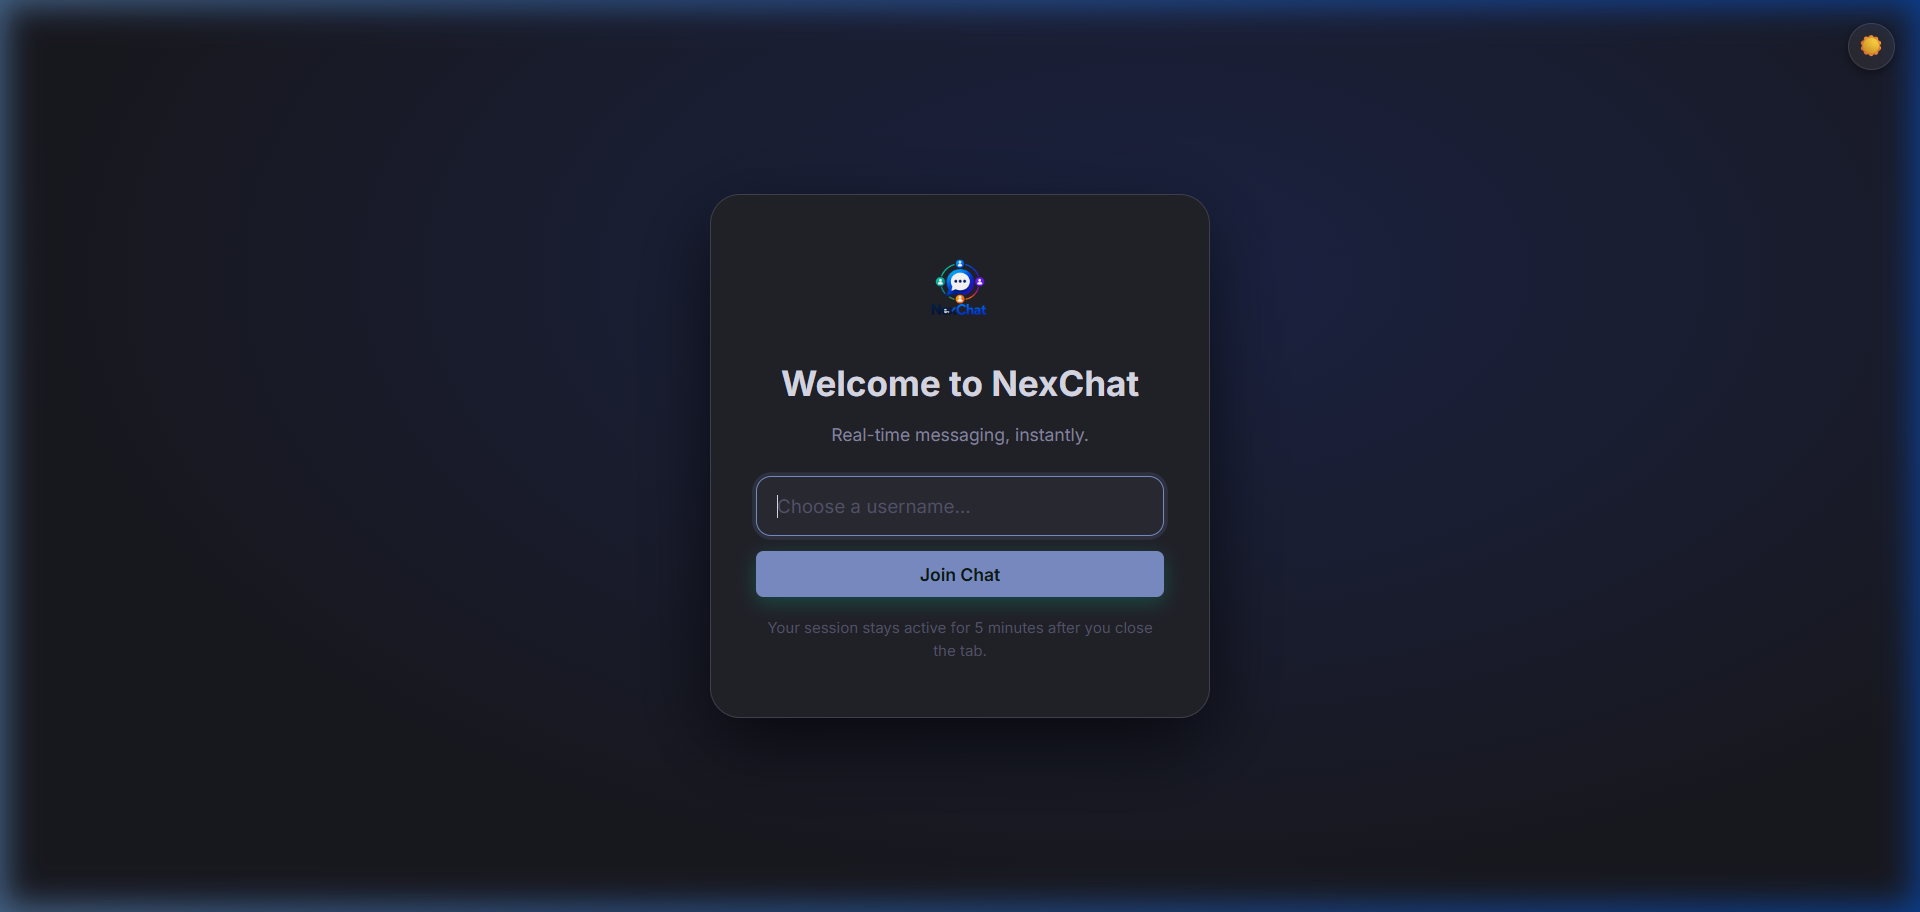
\includegraphics[width=0.8\textwidth]{1_login_page.png}
    \caption{Step 1: The login page featuring the custom logo and glassmorphism design.}
\end{figure}

\begin{figure}[ht]
    \centering
    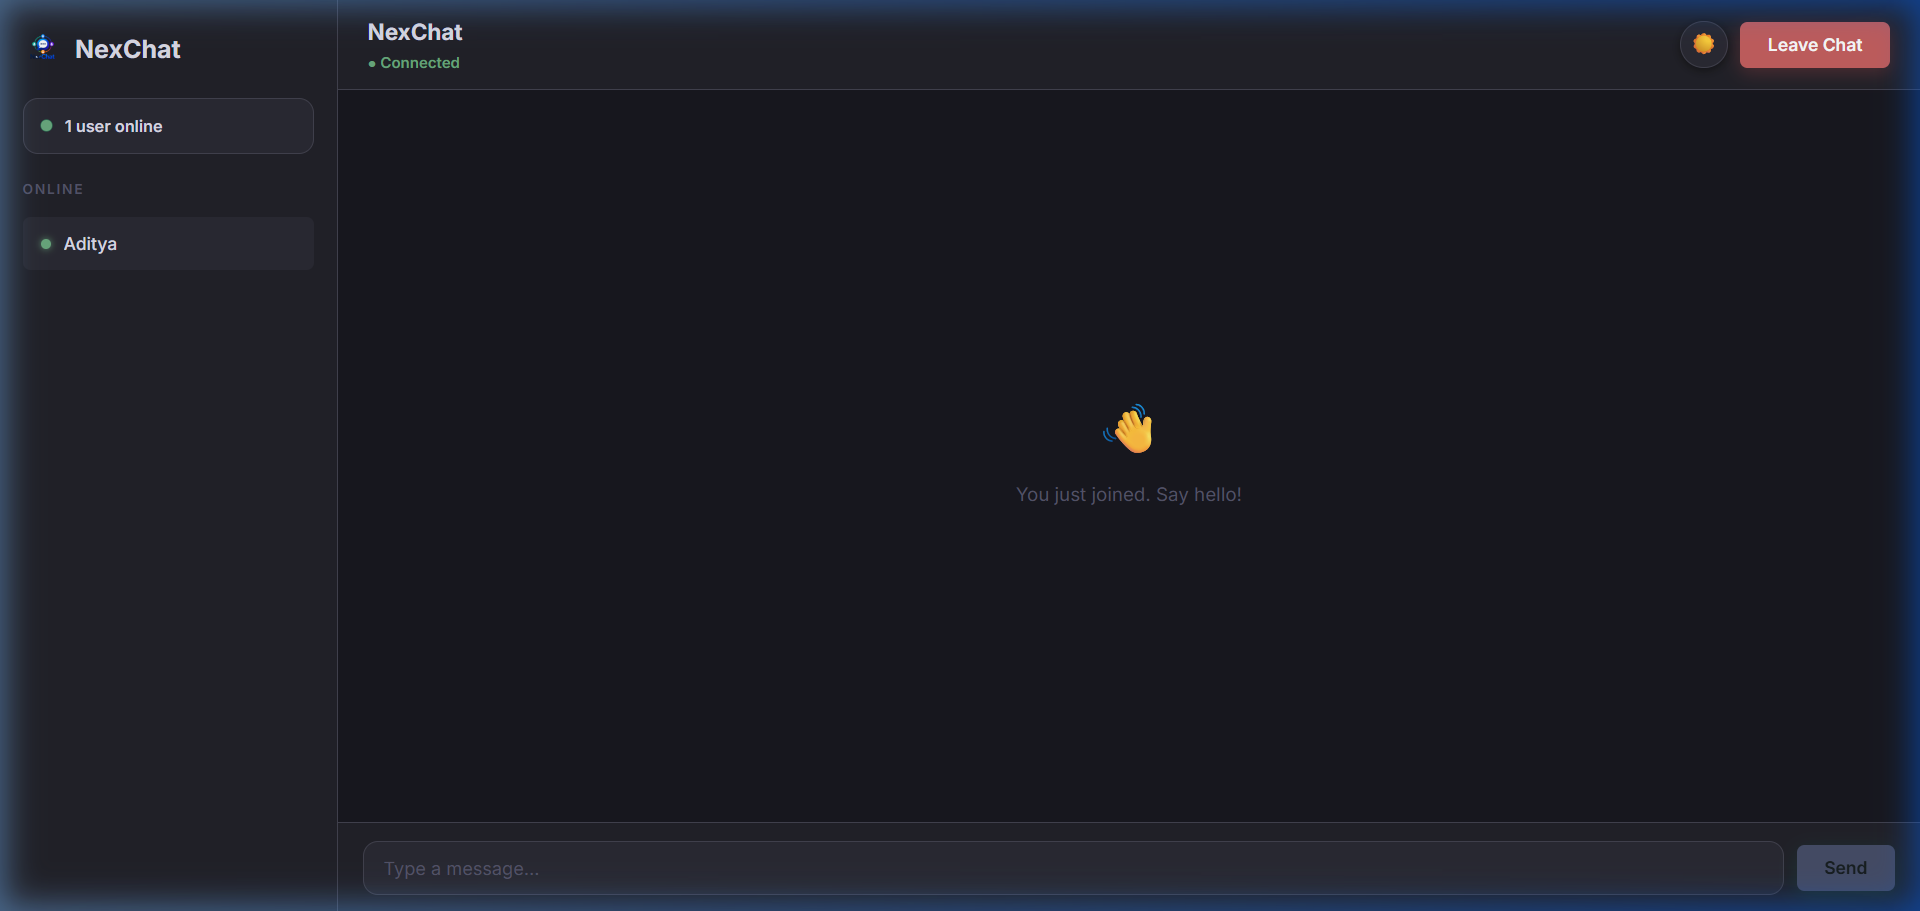
\includegraphics[width=0.8\textwidth]{2_chat_room_dark.png}
    \caption{Step 2a: The main chat room rendered in the default Dark Mode.}
\end{figure}

\begin{figure}[ht]
    \centering
    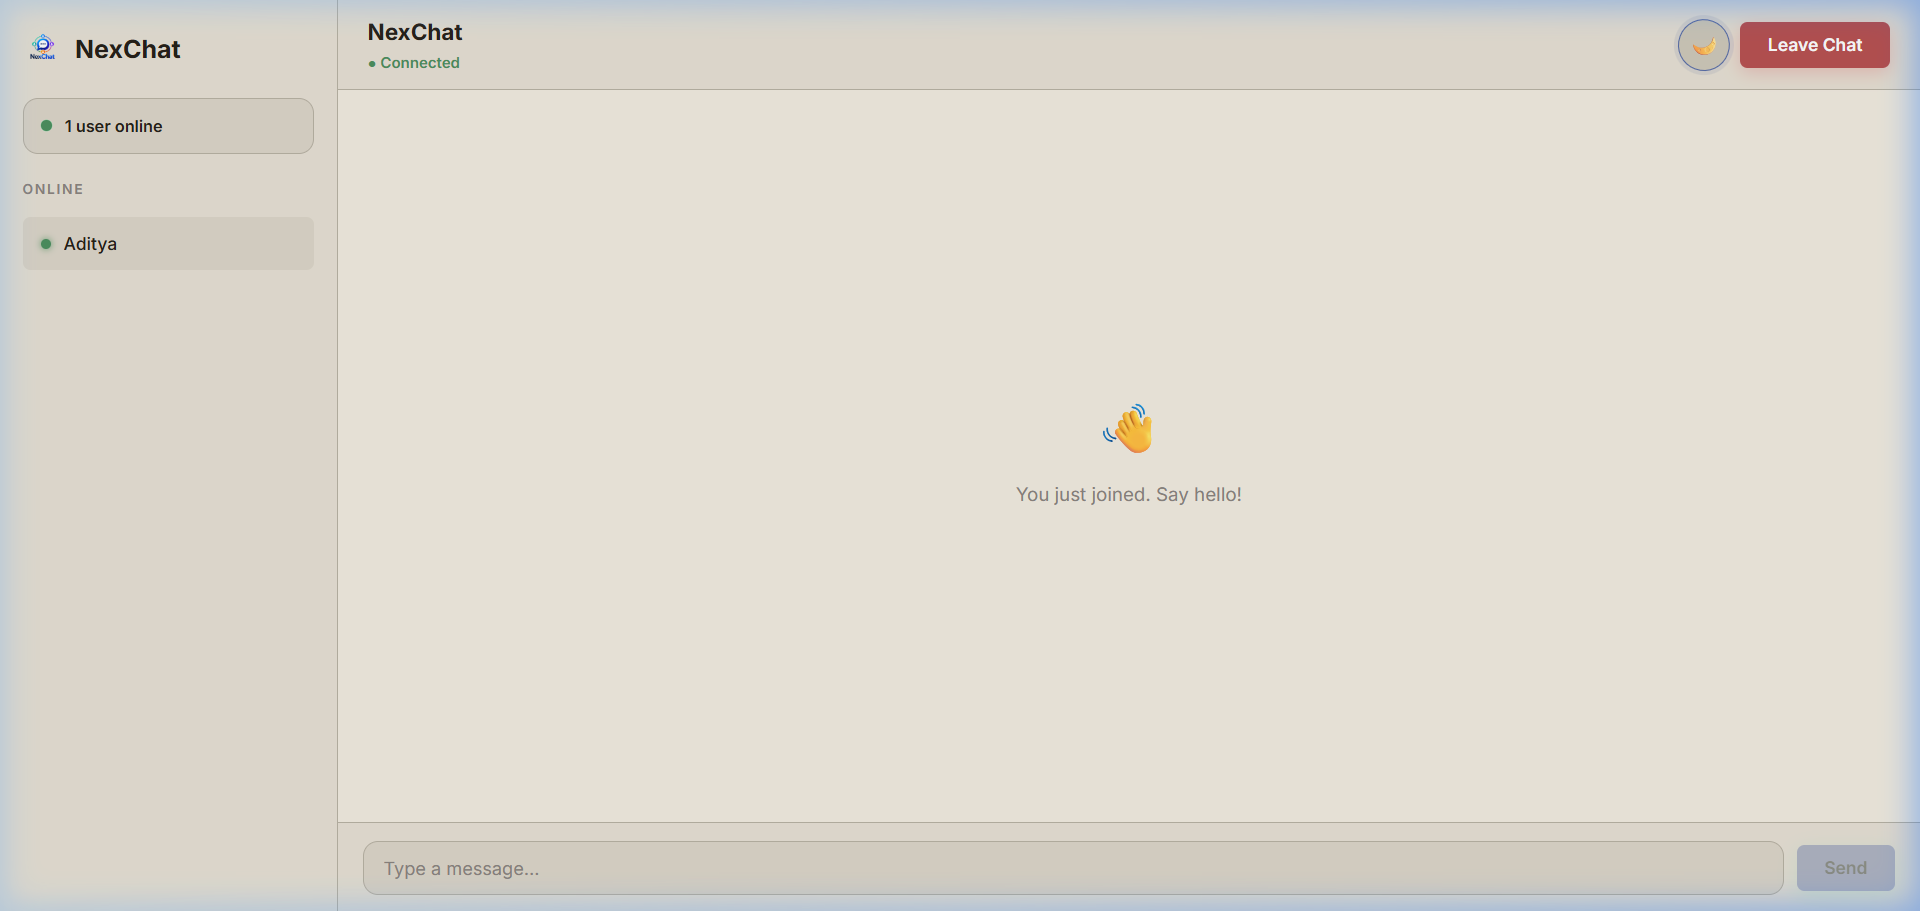
\includegraphics[width=0.8\textwidth]{2_chat_room_light.png}
    \caption{Step 2b: The main chat room seamlessly toggled to Light Mode.}
\end{figure}

\begin{figure}[ht]
    \centering
    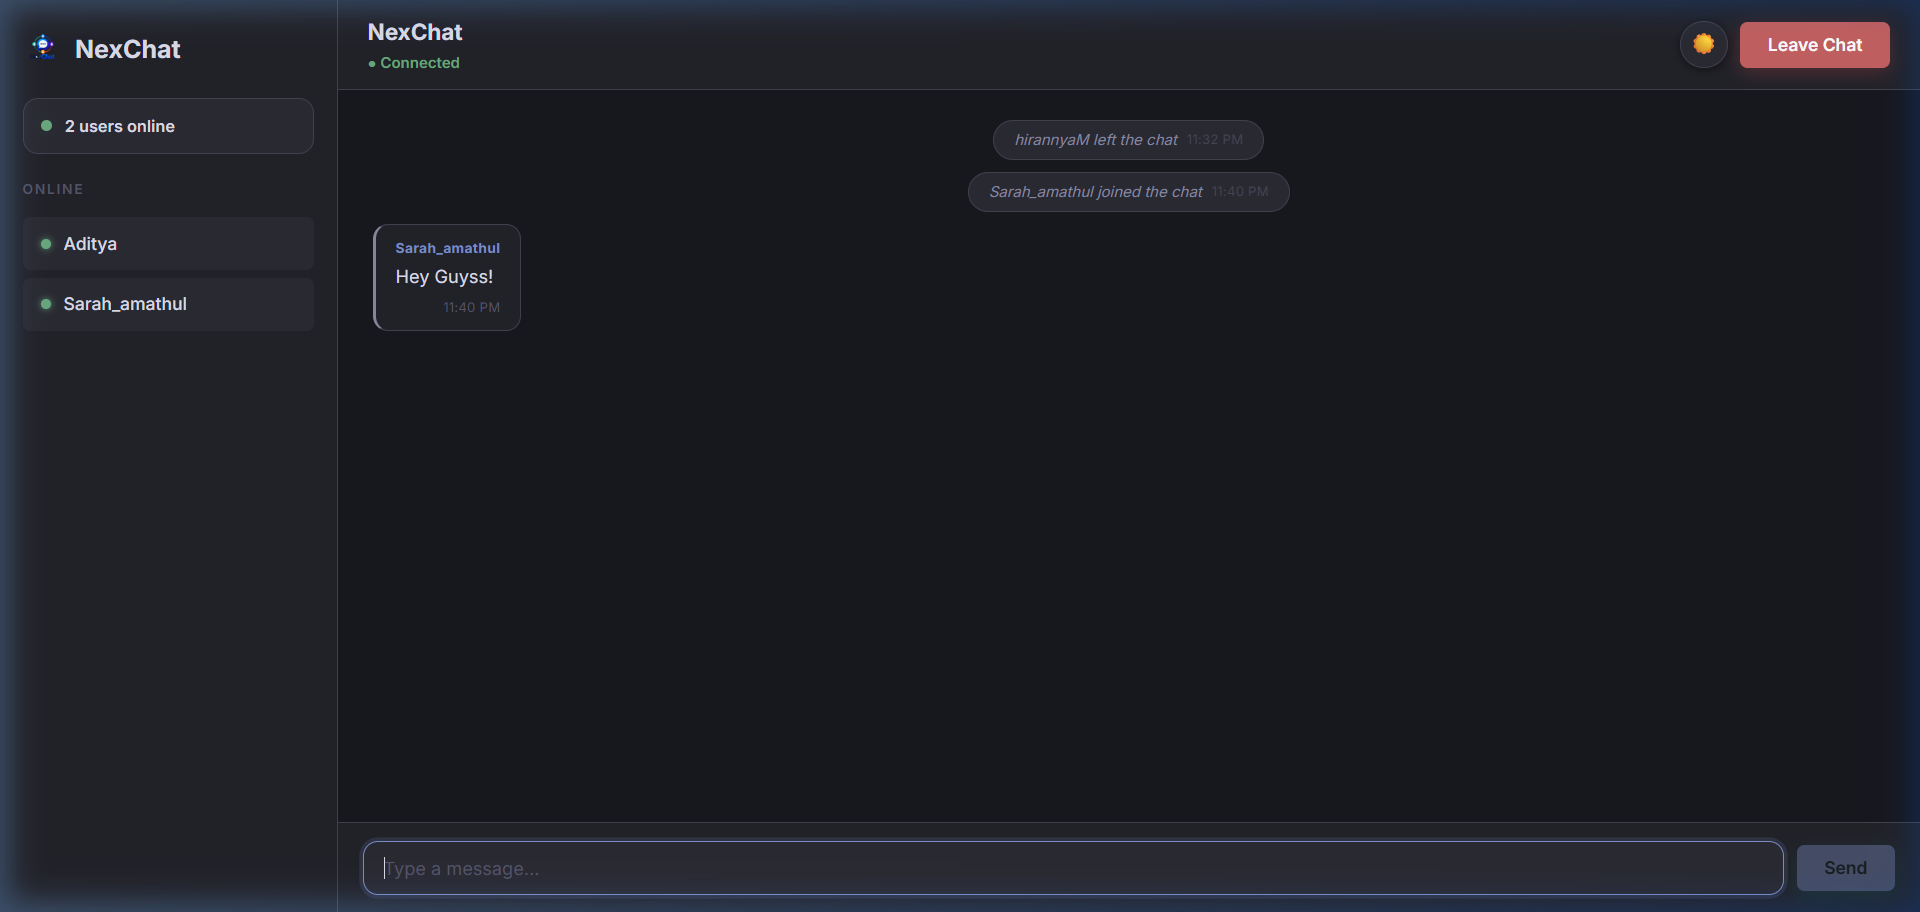
\includegraphics[width=0.8\textwidth]{3_all_users_online.png}
    \caption{Step 3: All four users connected and online in the chat room.}
\end{figure}

\begin{figure}[ht]
    \centering
    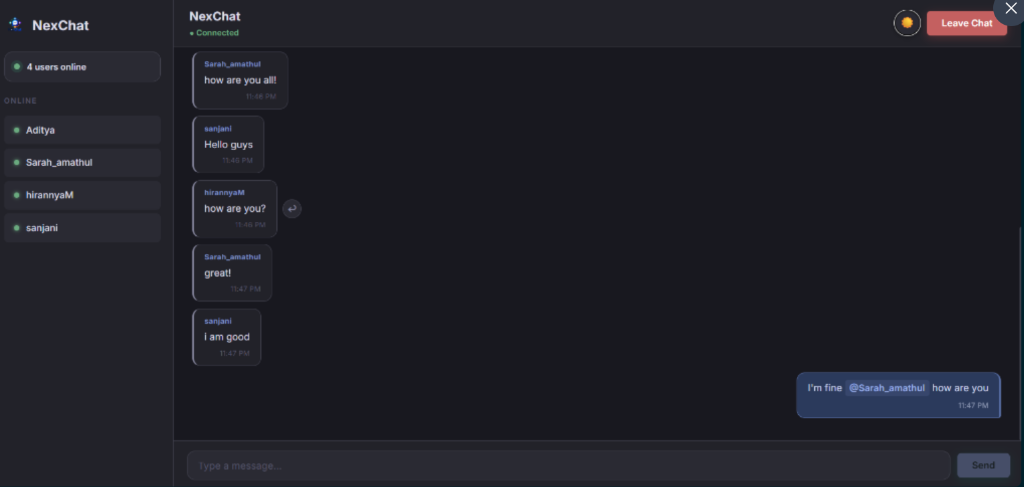
\includegraphics[width=0.8\textwidth]{4_all_messages.png}
    \caption{Step 4: Real messages exchanged between all four group members.}
\end{figure}

\begin{figure}[ht]
    \centering
    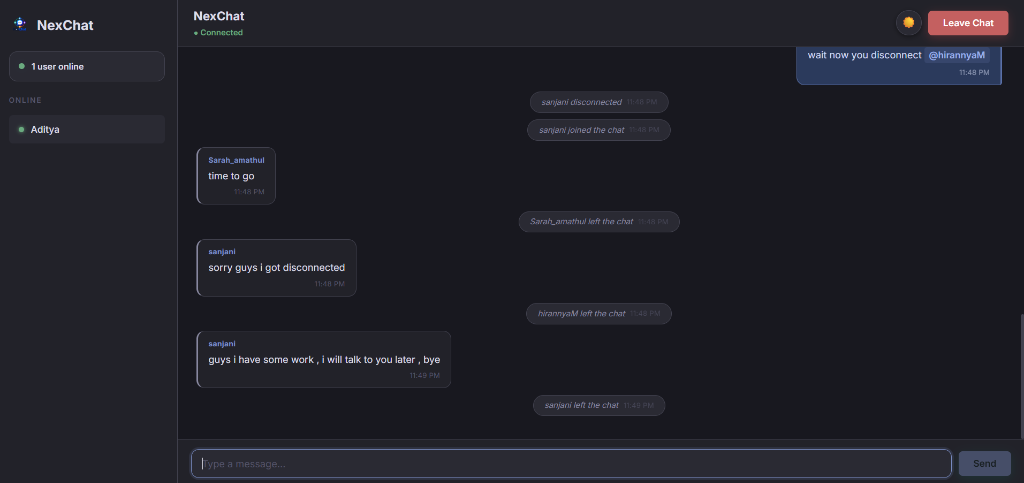
\includegraphics[width=0.8\textwidth]{5_disconnected.png}
    \caption{Step 5: System alerts as Sarah, Hirannya and Sanjani leave the chat one by one.}
\end{figure}

\clearpage
\section{Tech Stack Used}
The application utilizes a modern, decoupled technology stack designed for high concurrency and rapid development.

\subsection{Frontend (Client-Side)}
\begin{itemize}
    \item \textbf{Framework:} React 18
    \item \textbf{Build Tool:} Vite (for fast Hot Module Replacement and optimized builds)
    \item \textbf{Styling:} Vanilla CSS3 (Custom Design System, CSS Variables)
    \item \textbf{Networking:} Native WebSockets (Custom \texttt{useWebSocket} React hook)
    \item \textbf{State/Persistence:} React Hooks + Browser \texttt{localStorage}
    \item \textbf{Deployment:} Vercel Global CDN
\end{itemize}

\subsection{Backend (Server-Side)}
\begin{itemize}
    \item \textbf{Language:} Python 3
    \item \textbf{Framework:} FastAPI (Chosen for native async/await and WebSocket support)
    \item \textbf{Server:} Uvicorn (ASGI)
    \item \textbf{State Management:} In-Memory Python Dictionaries
    \item \textbf{Deployment:} Render Web Services
\end{itemize}

\section{Architecture}
NexChat follows a decoupled client-server architecture, enabling the frontend and backend to scale independently.

\subsection{WebSocket Communication Pipeline}
\begin{enumerate}
    \item \textbf{Connection Handshake:} When the React app loads the \texttt{ChatRoom} component, the \texttt{useWebSocket} hook instantly establishes a connection to the FastAPI \texttt{/ws} endpoint, passing a persistent UUID generated via \texttt{crypto.randomUUID()}.
    \item \textbf{Broadcasting Engine:} Every incoming message from a client is captured by the Python async loop, appended to a centralized \texttt{message\_history} array, and immediately mapped over all active connections via \texttt{asyncio.gather}. This ensures absolute zero-latency delivery to all connected clients.
\end{enumerate}

\subsection{System State and Resilience}
\begin{itemize}
    \item \textbf{Session Tracking:} The React frontend runs a background \texttt{setInterval} heartbeat every 60 seconds to update the session's timestamp in \texttt{localStorage}. 
    \item \textbf{Reconnection Logic:} On the backend, a \texttt{known\_sessions} dictionary tracks the exact time a user disconnected. If a user rejoins within the 5-minute grace period, the server identifies them as a returning user and securely dumps the entire recent message history back to them.
    \item \textbf{Cross-Origin Resource Sharing (CORS):} Middleware is explicitly configured in FastAPI to safely accept connections from the external Vercel frontend domain, bridging the gap between the two cloud environments.
\end{itemize}

\section{SSH Lab Deployment}
In addition to the public cloud deployment, NexChat was successfully hosted and demonstrated across four SSH virtual machines in a university lab environment (server IP: \texttt{10.1.75.51}), with each group member having a dedicated SSH port.

\subsection{Host Machine Setup (Aditya — Port 2217)}
One member hosted both the backend and the pre-built frontend:

\begin{enumerate}
    \item \textbf{Clone and install backend dependencies:}
    \begin{verbatim}
git clone https://github.com/Aj1359/Group-Chat-Application.git
cd Group-Chat-Application/backend
pip install -r requirements.txt
    \end{verbatim}

    \item \textbf{Start the backend permanently in the background:}
    \begin{verbatim}
nohup python3 -m uvicorn main:app \
  --host 0.0.0.0 --port 8000 > backend.log 2>&1 &
    \end{verbatim}

    \item \textbf{Build the frontend locally} (on personal laptop), pointing it to \texttt{localhost:8000}:
    \begin{verbatim}
echo "VITE_WS_URL=ws://localhost:8000/ws" > .env.production
npm run build
    \end{verbatim}

    \item \textbf{Copy the built \texttt{dist} folder to the SSH machine:}
    \begin{verbatim}
scp -P 2217 -r dist student@10.1.75.51:~/dist
    \end{verbatim}

    \item \textbf{Serve the frontend permanently in the background:}
    \begin{verbatim}
nohup python3 -m http.server 5173 \
  --directory ~/dist > frontend.log 2>&1 &
    \end{verbatim}
\end{enumerate}

\subsection{Connecting as a User (All Other Members)}
Since the university firewall blocked direct IP access on non-standard ports, all other members connected via SSH port forwarding (tunneling). Each member ran the following command on their \textbf{personal laptop}:
\begin{verbatim}
ssh -p <OWN_PORT> -L 5173:localhost:5173 \
  -L 8000:localhost:8000 student@10.1.75.51
\end{verbatim}

This creates a secure tunnel that maps \texttt{localhost:5173} and \texttt{localhost:8000} on their personal laptop to the host VM's running services. After logging in, each member simply opened their browser at \texttt{http://localhost:5173} and entered the chat room, all connected to the same backend.

\begin{table}[h]
\centering
\begin{tabular}{|l|c|l|}
\hline
\textbf{Member} & \textbf{SSH Port} & \textbf{Role} \\
\hline
Aditya Jha & 2217 & Host (Backend + Frontend) \\
Hirannya Mhaisbadwe & 2229 & User (SSH Tunnel) \\
Sarah Amathul Azeez & 2225 & User (SSH Tunnel) \\
Sanjani Kumari & 2221 & User (SSH Tunnel) \\
\hline
\end{tabular}
\caption{SSH port assignments for each group member}
\end{table}

\section{Conclusion}
The development of NexChat successfully integrated a responsive React frontend with a high-performance Python backend. By applying core computer systems concepts to solve complexities like WebSocket state management, multi-tab synchronization, cross-origin deployment, and SSH port-forwarding in a restricted university network, the group delivered a reliable, secure, and visually polished real-time communication platform.

\end{document}
